\subsection{More than one recurrence: partially heterologous markers}\label{ex:multiple_recurs_het}

\paragraph{Observed and phased alleles} In the simplest example a single allele is observed at one marker genotyped in an incident infection $t=0$ and in $t=1,2$ recurrent infections. Since we detect only one allele per infection we assume there is only one genotype per infection, s.t. $\bm{y} = \bm{a}$, e.g., 
\begin{align*}
    \bm{y} = 
    \begin{blockarray}{cl}\\
    \begin{block}{(c)l}
    \{A\} & t=0 \\
    \{T\} & t=1 \\
    \{T\} & t=2 \\
    \end{block}
    \end{blockarray},
    \hspace{1cm}
    \bm{a} = 
    \begin{blockarray}{cl}\\
    \begin{block}{(c)l}
    A & i=1 \\
    T & i=2 \\
    T & i=3 \\
    \end{block}
    \end{blockarray}.
\end{align*}

\paragraph{Relationship graphs and IBD partitions}
We sum over 12 relationship graphs, shown below in teal. For each graph, we sum over five IBD partitions $\ip_\RN{1}$ to $\ip_\RN{5}$ which can also be depicted as IBD graphs in grey.  
\begin{align*}
    \ip_\RN{1} &= \{\{1\},\{2\},\{3\}\}, \\
    \ip_\RN{2} &= \{\{1, 2, 3\}\}, \\
    \ip_\RN{3} &= \{\{2, 3\},\{2\}\}, \\
    \ip_\RN{4} &= \{\{1, 2\},\{3\}\}, \\
    \ip_\RN{5} &= \{\{1, 3\},\{2\}\}. \\
\end{align*}
 
\begin{center}
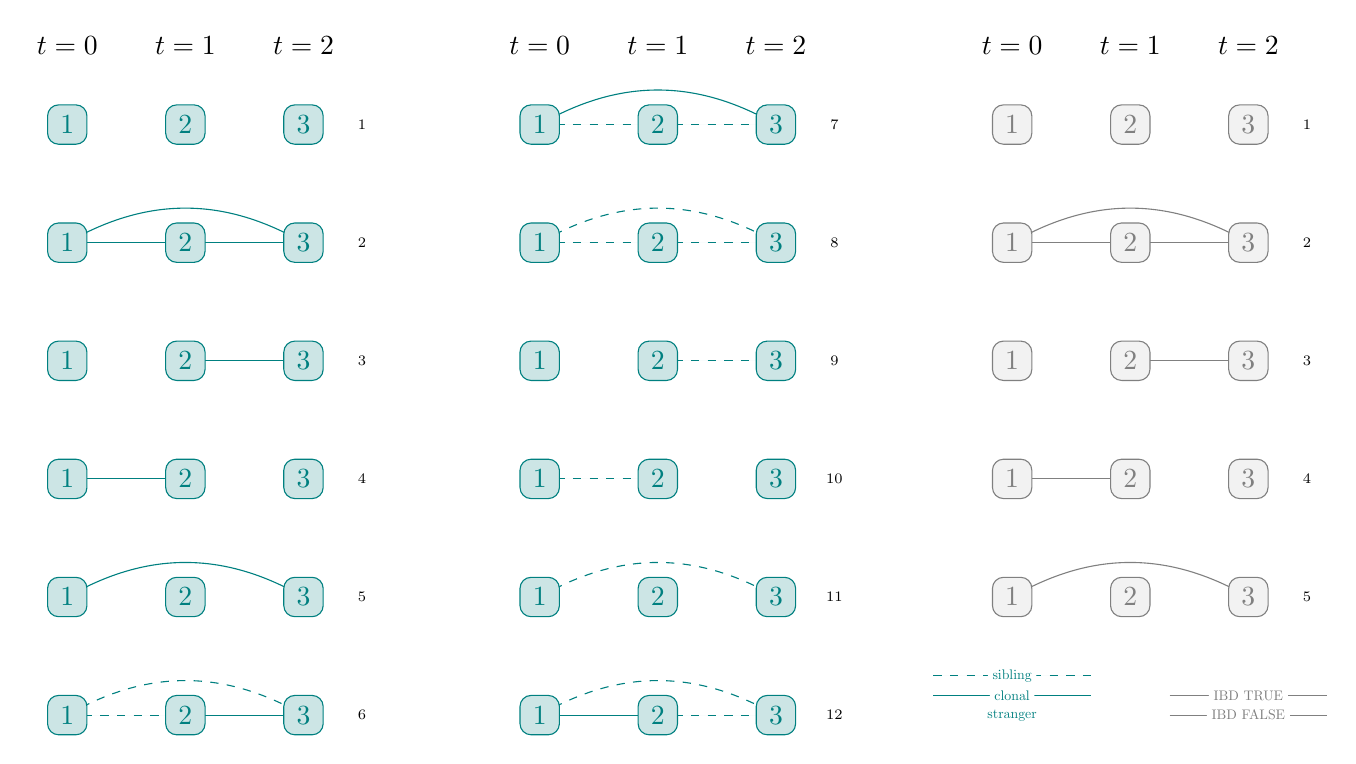
\begin{tikzpicture}
    \tikzstyle{geno} = [draw, rectangle, rounded corners, minimum height=0.5cm, minimum width=0.5cm, color = teal, 
    fill = teal!20]
    
    \tikzstyle{ibd} = [draw, rectangle, rounded corners, minimum height=0.5cm, minimum width=0.5cm, color = gray, 
    fill = gray!10]
    
    \node at (0,1) {$t=0$};
    \node at (1.5,1) {$t=1$};
    \node at (3,1) {$t=2$}; 
    \node at (6,1) {$t=0$};
    \node at (7.5,1) {$t=1$};
    \node at (9,1) {$t=2$}; 
    \node at (12,1) {$t=0$};
    \node at (13.5,1) {$t=1$};
    \node at (15,1) {$t=2$}; 
    \node[scale = 0.75] at (3.75,0) {$\rg_\RN{1}$};
    \node[scale = 0.75] at (3.75,-1.5) {$\rg_\RN{2}$};
    \node[scale = 0.75] at (3.75,-3) {$\rg_\RN{3}$}; 
    \node[scale = 0.75] at (3.75,-4.5) {$\rg_\RN{4}$};
    \node[scale = 0.75] at (3.75,-6) {$\rg_\RN{5}$};
    \node[scale = 0.75] at (3.75,-7.5) {$\rg_\RN{6}$}; 
    \node[scale = 0.75] at (9.75,0) {$\rg_\RN{7}$};
    \node[scale = 0.75] at (9.75,-1.5) {$\rg_\RN{8}$};
    \node[scale = 0.75] at (9.75,-3) {$\rg_\RN{9}$}; 
    \node[scale = 0.75] at (9.75,-4.5) {$\rg_\RN{10}$};
    \node[scale = 0.75] at (9.75,-6) {$\rg_\RN{11}$};
    \node[scale = 0.75] at (9.75,-7.5) {$\rg_\RN{12}$}; 
    \node[scale = 0.75] at (15.75,0) {$\ip_\RN{1}$};
    \node[scale = 0.75] at (15.75,-1.5) {$\ip_\RN{2}$};
    \node[scale = 0.75] at (15.75,-3) {$\ip_\RN{3}$}; 
    \node[scale = 0.75] at (15.75,-4.5) {$\ip_\RN{4}$};
    \node[scale = 0.75] at (15.75,-6) {$\ip_\RN{5}$};
 
    % Graph 1
    \node[geno] at (0,0) {$1$};
    \node[geno] at (1.5,0) {$2$};
    \node[geno] at (3,0) {$3$}; 
    
    % Graph 2
    \path[geno, bend left] (0,-1.5) edge (3,-1.5);
    \draw[geno] (0,-1.5) -- (1.5,-1.5);
    \draw[geno] (1.5,-1.5) -- (3,-1.5);
    \node[geno] at (0,-1.5) {$1$};
    \node[geno] at (1.5,-1.5) {$2$};
    \node[geno] at (3,-1.5) {$3$}; 
    
    % Graph 3
    \draw[geno](1.5,-3) -- (3,-3);
    \node[geno] at (0,-3) {$1$};
    \node[geno] at (1.5,-3) {$2$};
    \node[geno] at (3,-3) {$3$}; 
    
    % Graph 4
    \draw[geno] (0,-4.5) -- (1.5,-4.5);
    \node[geno] at (0,-4.5) {$1$};
    \node[geno] at (1.5,-4.5) {$2$};
    \node[geno] at (3,-4.5) {$3$}; 
    
    % Graph 5
    \path[geno, bend left](0,-6) edge (3,-6);
    \node[geno] at (0,-6) {$1$};
    \node[geno] at (1.5,-6) {$2$};
    \node[geno] at (3,-6) {$3$}; 
    
    % Graph 6
    \path[geno, dashed, bend left] (0,-7.5) edge (3,-7.5);
    \draw[geno, dashed] (0,-7.5) -- (1.5,-7.5);
    \draw[geno] (1.5,-7.5) -- (3,-7.5);
    \node[geno] at (0,-7.5) {$1$};
    \node[geno] at (1.5,-7.5) {$2$};
    \node[geno] at (3,-7.5) {$3$}; 
    
    % Graph 7
    \path[geno, bend left] (6,0) edge (9,0);
    \draw[geno, dashed] (6,0) -- (7.5,0);
    \draw[geno, dashed] (7.5,0) -- (9,0);
    \node[geno] at (6,0) {$1$};
    \node[geno] at (7.5,0) {$2$};
    \node[geno] at (9,0) {$3$}; 
    
    % Graph 8
    \path[geno, dashed, bend left] (6,-1.5) edge (9,-1.5);
    \draw[geno, dashed] (6,-1.5) -- (7.5,-1.5);
    \draw[geno, dashed] (7.5,-1.5) -- (9,-1.5);
    \node[geno] at (6,-1.5) {$1$};
    \node[geno] at (7.5,-1.5) {$2$};
    \node[geno] at (9,-1.5) {$3$}; 
    
    % Graph 9
    \draw[geno, dashed] (7.5,-3) -- (9,-3);
    \node[geno] at (6,-3) {$1$};
    \node[geno] at (7.5,-3) {$2$};
    \node[geno] at (9,-3) {$3$}; 
    
    % Graph 10
    \draw[geno, dashed] (6,-4.5) -- (7.5,-4.5);
    \node[geno] at (6,-4.5) {$1$};
    \node[geno] at (7.5,-4.5) {$2$};
    \node[geno] at (9,-4.5) {$3$}; 
    
    % Graph 11
    \path[geno, dashed, bend left] (6,-6) edge (9,-6);
    \node[geno] at (6,-6) {$1$};
    \node[geno] at (7.5,-6) {$2$};
    \node[geno] at (9,-6) {$3$}; 
    
    % Graph 12
    \path[geno, dashed, bend left] (6,-7.5) edge (9,-7.5);
    \draw[geno] (6,-7.5) -- (7.5,-7.5);
    \draw[geno, dashed] (7.5,-7.5) -- (9,-7.5);
    \node[geno] at (6,-7.5) {$1$};
    \node[geno] at (7.5,-7.5) {$2$};
    \node[geno] at (9,-7.5) {$3$}; 
    
    % Graph 1
    \node[ibd] at (12,0) {$1$};
    \node[ibd] at (13.5,0) {$2$};
    \node[ibd] at (15,0) {$3$}; 
    
    % Graph 2
    \path[ibd, bend left] (12,-1.5) edge (15,-1.5);
    \draw[ibd] (12,-1.5) -- (13.5,-1.5);
    \draw[ibd] (13.5,-1.5) -- (15,-1.5);
    \node[ibd] at (12,-1.5) {$1$};
    \node[ibd] at (13.5,-1.5) {$2$};
    \node[ibd] at (15,-1.5) {$3$}; 
    
    % Graph 3
    \draw[ibd] (13.5,-3) -- (15,-3);
    \node[ibd] at (12,-3) {$1$};
    \node[ibd] at (13.5,-3) {$2$};
    \node[ibd] at (15,-3) {$3$}; 
    
    % Graph 4
    \draw[ibd] (12,-4.5) -- (13.5,-4.5);
    \node[ibd] at (12,-4.5) {$1$};
    \node[ibd] at (13.5,-4.5) {$2$};
    \node[ibd] at (15,-4.5) {$3$}; 
    
    % Graph 5
    \path[ibd, bend left] (12,-6) edge (15,-6);
    \node[ibd] at (12,-6) {$1$};
    \node[ibd] at (13.5,-6) {$2$};
    \node[ibd] at (15,-6) {$3$}; 

    % Legend
    \draw[dashed, geno] (11,-7) -- (13,-7) 
    node[scale=0.5, midway, fill=white]{sibling};
    \draw[geno] (11,-7.25) -- (13,-7.25) 
    node[scale=0.5, midway, fill=white]{clonal};
    \path (11,-7.5) -- (13,-7.5) 
    node[scale=0.5, midway, fill=white, text = teal]{stranger};
    \draw[ibd] (14,-7.25) -- (16,-7.25) 
    node[scale=0.5, midway, fill=white]{IBD TRUE};
    \path[ibd] (14,-7.5) -- (16,-7.5) 
    node[scale=0.5, midway, fill=white]{IBD FALSE};
\end{tikzpicture}
\end{center}


\paragraph{Likelihood} 
Remembering that in linear algebra $(CBA)^T = (A^TB^TC^T)$, 
\small
\begin{align*}
&\mathbb{P}(\bm{y}|\bm{s})\forall\bm{s}\in\{L,I,C\} \times \{L,I,C\} = 
\mathbb{P}(\bm{a}|\bm{s})\forall\bm{s}\in\{L,I,C\} \times \{L,I,C\}, \\
&=\underbrace{ 
    \begin{blockarray}{cl}
    \bm{a} \\
    \begin{block}{(c)l}
    \sfrac{5}{24}f(A)f(T)^2 + \sfrac{9}{48} f(A)f(T) & LL \\
    \sfrac{2}{5}f(A)f(T)^2 + \sfrac{3}{10}f(A)f(T) & IL \\ 
    \sfrac{1}{2}f(A)f(T)^2 & LI \\ 
    \sfrac{1}{2}f(A)f(T) & LC \\ 
    0 & CL \\
    f(A)f(T)^2 & II \\
    0 & CC \\
    f(A)f(T) & IC \\
    0 & CI \\
    \end{block}
    \end{blockarray},
    }_{\mathclap{\mathbb{P}(\bm{a}|\bm{s})\forall\bm{s}\in\{L,I,C\} \times \{L,I,C\}}}
    \\
    &=\underbrace{
    \begin{blockarray}{ccccccccccccl}
        \rg_\RN{1} & \rg_\RN{2} &
        \rg_\RN{3} & \rg_\RN{4} &
        \rg_\RN{5} & \rg_\RN{6} &
        \rg_\RN{7} & \rg_\RN{8} &
        \rg_\RN{9} & \rg_\RN{10} &
        \rg_\RN{11} & \rg_\RN{12} & \\
        \begin{block}{(cccccccccccc)l}
          \sfrac{1}{12} & \sfrac{1}{12} & \sfrac{1}{12} &
          \sfrac{1}{12} & \sfrac{1}{12} & \sfrac{1}{12} &\sfrac{1}{12} & \sfrac{1}{12} & \sfrac{1}{12} &\sfrac{1}{12} & \sfrac{1}{12} & \sfrac{1}{12} 
          & LL \\
          \sfrac{1}{5}&0&\sfrac{1}{5}&
          0&\sfrac{1}{5}&0&0&0&\sfrac{1}{5}&0&\sfrac{1}{5}&0
          & IL \\
          \sfrac{1}{3}&0&0&\sfrac{1}{3}&
          0&0&0&0&0&\sfrac{1}{3}&0&0
          & LI \\
          0&\sfrac{1}{3}&\sfrac{1}{3}&0&
          0&\sfrac{1}{3}&0&0&0&0&0&0
          & LC \\
          0&\sfrac{1}{3}&0&\sfrac{1}{3}&
          0&0&0&0&0&0&0&\sfrac{1}{3}
          & CL \\
          1&0&0&0&0&0&0&0&0&0&0&0& II \\
          0&1&0&0&0&0&0&0&0&0&0&0& CC \\
          0&0&1&0&0&0&0&0&0&0&0&0& IC \\
          0&0&0&1&0&0&0&0&0&0&0&0& CI \\
        \end{block}
        \end{blockarray} 
        }_{_{\mathclap{\mathbb{P}(\rg|\bm{s}) \forall \rg\in\RG, \bm{s}\in\{L,I,C\} \times \{L,I,C\}}}}
    \times 
    \underbrace{
    \begin{blockarray}{cl}
    \bm{a} \\
    \begin{block}{(c)l}
    f(A)f(T)^2 & \rg_\RN{1} \\
    0 & \rg_\RN{2} \\ 
    f(A)f(T) & \rg_\RN{3} \\ 
    0 & \rg_\RN{4} \\ 
    0 & \rg_\RN{5} \\
    \sfrac{1}{2} f(A)f(T) & \rg_\RN{6} \\
    0 & \rg_\RN{7} \\
    \sfrac{1}{4} f(A)f(T) & \rg_\RN{8} \\
    \sfrac{1}{2} f(A)f(T)(f(T) + 1)  & \rg_\RN{9} \\
    \sfrac{1}{2} f(A)f(T)^2 &\rg_\RN{10} \\
    \sfrac{1}{2} f(A)f(T)^2 &\rg_\RN{11} \\
    0 &\rg_\RN{12} \\
    \end{block}
    \end{blockarray}
    }_{\mathclap{\mathbb{P}(\bm{a}|\bm{s})\forall\bm{s}\in\{L,I,C\} \times \{L,I,C\}}}, \\
    &=
    \underbrace{
    \begin{blockarray}{ccccccccccccl}
        \rg_\RN{1} & \rg_\RN{2} &
        \rg_\RN{3} & \rg_\RN{4} &
        \rg_\RN{5} & \rg_\RN{6} &
        \rg_\RN{7} & \rg_\RN{8} &
        \rg_\RN{9} & \rg_\RN{10} &
        \rg_\RN{11} & \rg_\RN{12} & \\
        \begin{block}{(cccccccccccc)l}
          \sfrac{1}{12} & \sfrac{1}{12} & \sfrac{1}{12} &
          \sfrac{1}{12} & \sfrac{1}{12} & \sfrac{1}{12} &\sfrac{1}{12} & \sfrac{1}{12} & \sfrac{1}{12} &\sfrac{1}{12} & \sfrac{1}{12} & \sfrac{1}{12} 
          & LL \\
          \sfrac{1}{5}&0&\sfrac{1}{5}&
          0&\sfrac{1}{5}&0&0&0&\sfrac{1}{5}&0&\sfrac{1}{5}&0
          & IL \\
          \sfrac{1}{3}&0&0&\sfrac{1}{3}&
          0&0&0&0&0&\sfrac{1}{3}&0&0
          & LI \\
          0&\sfrac{1}{3}&\sfrac{1}{3}&0&
          0&\sfrac{1}{3}&0&0&0&0&0&0
          & LC \\
          0&\sfrac{1}{3}&0&\sfrac{1}{3}&
          0&0&0&0&0&0&0&\sfrac{1}{3}
          & CL \\
          1&0&0&0&0&0&0&0&0&0&0&0& II \\
          0&1&0&0&0&0&0&0&0&0&0&0& CC \\
          0&0&1&0&0&0&0&0&0&0&0&0& IC \\
          0&0&0&1&0&0&0&0&0&0&0&0& CI \\
        \end{block}
        \end{blockarray} 
        }_{_{\mathclap{\mathbb{P}(\rg|\bm{s}) \forall \rg\in\RG, \bm{s}\in\{L,I,C\} \times \{L,I,C\}}}}
    \times \quad \\
    &\; \underbrace{ 
    \begin{blockarray}{cccccl}
    \ip_\RN{1} & \ip_\RN{2} & \ip_\RN{3} & 
    \ip_\RN{4} & \ip_\RN{5} \\
    \begin{block}{(ccccc)l}
    1&0&0&0&0&\rg_\RN{1} \\
    0&1&0&0&0&\rg_\RN{2} \\
    0&0&1&0&0&\rg_\RN{3} \\
    0&0&0&1&0&\rg_\RN{4} \\
    0&0&0&0&1&\rg_\RN{5} \\
    0&\sfrac{1}{2}&\sfrac{1}{2}&0&0&\rg_\RN{6} \\
    0&\sfrac{1}{2}&0&0&\sfrac{1}{2}&\rg_\RN{7} \\
    0&\sfrac{1}{4}&\sfrac{1}{4}&\sfrac{1}{4}&\sfrac{1}{4}&\rg_\RN{8} \\
    \sfrac{1}{2}&0&\sfrac{1}{2}&0&0&\rg_\RN{9} \\
    \sfrac{1}{2}&0&0&\sfrac{1}{2}&0&\rg_\RN{10} \\
    \sfrac{1}{2}&0&0&0&\sfrac{1}{2}&\rg_\RN{11} \\
    0&\sfrac{1}{2}&0&\sfrac{1}{2}&0&\rg_\RN{12} \\
    \end{block}
    \end{blockarray}
    }_{\mathclap{\mathbb{P}(\ip|\rg)\forall\ip\in\IP,\rg\in\RG}}
    \times \quad
    \underbrace{ 
    \begin{blockarray}{cl}
    \bm{a}_{\cdot 1} \\
    \begin{block}{(c)l}
    f(A)f(T)^2 & \ip_\RN{1}=\{\{1\},\{2\},\{3\}\} \\
    0 & \ip_\RN{2} = \{\{1, 2, 3\}\} \\ 
    f(A)f(T) & \ip_\RN{3} = \{\{2, 3\},\{2\}\}\\ 
    0 & \ip_\RN{4} = \{\{1, 2\},\{3\}\}\\ 
    0 & \ip_\RN{5} = \{\{1, 3\},\{2\}\}\\
    \end{block}
    \end{blockarray}
    }_{\mathclap{\mathbb{P}(\bm{a}_{\cdot j}|\ip)\forall\bm{a}_{\cdot j}\in\bm{a},\ip\in\IP}}.
\end{align*}


\pagebreak
\paragraph{Posterior}
For a uniform prior on $\bm{s}\in\{L,I,C\}$, 
$\mathbb{P}(\bm{a}) = \tfrac{253}{360}f(A)f(T)^2 + \tfrac{53}{80} f(A)f(T)$ and
\begin{align*}
    \mathbb{P}(s_1 | \bm{y}) \forall s_1\in\{L,I,C\} 
    &=
    {\underbrace{\Big( \tfrac{253}{360}f(A)f(T)^2 + \tfrac{53}{80} f(A)f(T) \Big)
    }_{\mathclap{\mathbb{P}(\bm{y})}}}^{-1} \times \tfrac{1}{3} \times 
    \underbrace{ 
    \begin{blockarray}{cl}
    \begin{block}{(c)l}
    \sfrac{17}{24}f(A)f(T)^2 + \sfrac{11}{16} f(A)f(T) & L \\
    \sfrac{7}{5}f(A)f(T)^2 + \sfrac{13}{10}f(A)f(T) & I \\ 
    0 & C \\
    \end{block}
    \end{blockarray}
    }_{\mathclap{\mathbb{P}(\bm{y}|s_1)\forall s_1\in\{L,I,C\}}}, 
\end{align*}    
    
    
\begin{align*}    
    \mathbb{P}(s_2 | \bm{y}) \forall s_2\in\{L,I,C\} 
    &= 
    {\underbrace{\Big( \tfrac{253}{360}f(A)f(T)^2 + \tfrac{53}{80} f(A)f(T) \Big)
    }_{\mathclap{\mathbb{P}(\bm{y})}}}^{-1} \times \tfrac{1}{3} \times 
    \underbrace{ 
    \begin{blockarray}{cl}
    \begin{block}{(c)l}
    \sfrac{73}{120}f(A)f(T)^2 + \sfrac{39}{80} f(A)f(T) & L \\
    \sfrac{3}{2}f(A)f(T)^2 & I \\ 
    \sfrac{3}{2}f(A)f(T) & C \\
    \end{block}
    \end{blockarray}
    }_{\mathclap{\mathbb{P}(\bm{y}|s_2)\forall s_2\in\{L,I,C\}}}.
\end{align*}

\subsection{More than one recurrence: exclusively homologous markers}\label{ex:multiple_recurs_hom}

If instead $\bm{y} = (\{A\}, \{A\}, \{A\})^{T}$, $\mathbb{P}(\bm{y}|\bm{s}) = \mathbb{P}(\bm{a}|\bm{s})$, which for $\bm{s}=II$ and $\bm{s}=CC$
\begin{align*}
&=\underbrace{ 
    \begin{blockarray}{cl}
    \bm{a} \\
    \begin{block}{(c)l}
    f(A)^3 & II \\
    f(A) & CC \\
    \end{block}
    \end{blockarray},
    }_{\mathclap{\mathbb{P}(\bm{a}|\bm{s})\text{ for } II \text{ and } CC}}
    \\
    &=\underbrace{
    \begin{blockarray}{ccccccccccccl}
        \rg_\RN{1} & \rg_\RN{2} &
        \rg_\RN{3} & \rg_\RN{4} &
        \rg_\RN{5} & \rg_\RN{6} &
        \rg_\RN{7} & \rg_\RN{8} &
        \rg_\RN{9} & \rg_\RN{10} &
        \rg_\RN{11} & \rg_\RN{12} & \\
        \begin{block}{(cccccccccccc)l}
          1&0&0&0&0&0&0&0&0&0&0&0& II \\
          0&1&0&0&0&0&0&0&0&0&0&0& CC \\
        \end{block}
        \end{blockarray} 
        }_{_{\mathclap{\mathbb{P}(\rg|\bm{s}) \text{ for } II \text{ and } CC}}}
    \times 
    \underbrace{
    \begin{blockarray}{cl}
    \bm{a} \\
    \begin{block}{(c)l}
    f(A)^3 & \rg_\RN{1} \\
    f(A) & \rg_\RN{2} \\ 
    f(A)^2 & \rg_\RN{3} \\ 
    f(A)^2 & \rg_\RN{4} \\ 
    f(A)^2 & \rg_\RN{5} \\
    \sfrac{1}{2}(f(A)^2 + f(A)) & \rg_\RN{6} \\
    \sfrac{1}{2}(f(A)^2 + f(A)) & \rg_\RN{7} \\
    \sfrac{1}{4}(3f(A)^2 + f(A)) & \rg_\RN{8} \\
    \sfrac{1}{2}(f(A)^3 + f(A)^2)  & \rg_\RN{9} \\
    \sfrac{1}{2}(f(A)^3 + f(A)^2) &\rg_\RN{10} \\
    \sfrac{1}{2}(f(A)^3 + f(A)^2) &\rg_\RN{11} \\
    \sfrac{1}{2}(f(A)^2 + f(A)) &\rg_\RN{12} \\
    \end{block}
    \end{blockarray}
    }_{\mathclap{\mathbb{P}(\bm{a}|\rg)\forall\rg\in\RG}}, \\
    &= \mathbb{P}(\rg|\bm{s}) \text{ for } II \text{ and } CC \times 
    \underbrace{ 
    \begin{blockarray}{cccccl}
    \ip_\RN{1} & \ip_\RN{2} & \ip_\RN{3} & 
    \ip_\RN{4} & \ip_\RN{5} \\
    \begin{block}{(ccccc)l}
    1&0&0&0&0&\rg_\RN{1} \\
    0&1&0&0&0&\rg_\RN{2} \\
    0&0&1&0&0&\rg_\RN{3} \\
    0&0&0&1&0&\rg_\RN{4} \\
    0&0&0&0&1&\rg_\RN{5} \\
    0&\sfrac{1}{2}&\sfrac{1}{2}&0&0&\rg_\RN{6} \\
    0&\sfrac{1}{2}&0&0&\sfrac{1}{2}&\rg_\RN{7} \\
    0&\sfrac{1}{4}&\sfrac{1}{4}&\sfrac{1}{4}&\sfrac{1}{4}&\rg_\RN{8} \\
    \sfrac{1}{2}&0&\sfrac{1}{2}&0&0&\rg_\RN{9} \\
    \sfrac{1}{2}&0&0&\sfrac{1}{2}&0&\rg_\RN{10} \\
    \sfrac{1}{2}&0&0&0&\sfrac{1}{2}&\rg_\RN{11} \\
    0&\sfrac{1}{2}&0&\sfrac{1}{2}&0&\rg_\RN{12} \\
    \end{block}
    \end{blockarray}
    }_{\mathclap{\mathbb{P}(\ip|\rg)\forall\ip\in\IP,\rg\in\RG}}
    \times \quad
    \underbrace{ 
    \begin{blockarray}{cl}
    \bm{a}_{\cdot 1} \\
    \begin{block}{(c)l}
    f(A)^3 & \ip_\RN{1}=\{\{1\},\{2\},\{3\}\}\\
    f(A) & \ip_\RN{2}=\{\{1, 2, 3\}\} \\ 
    f(A)^2 & \ip_\RN{3}=\{\{2, 3\},\{2\}\} \\ 
    f(A)^2 & \ip_\RN{4}=\{\{1, 2\},\{3\}\} \\ 
    f(A)^2 & \ip_\RN{5}=\{\{1, 3\},\{2\}\} \\
    \end{block}
    \end{blockarray}.
    }_{\mathclap{\mathbb{P}(\bm{a}_{\cdot j}|\ip)\forall\bm{a}_{\cdot j}\in\bm{a},\ip\in\IP}}
\end{align*}
